\documentclass[10pt]{article}

\usepackage[T1]{fontenc}
\usepackage{newtxtext,newtxmath}
\usepackage[margin=0.78in]{geometry}
\usepackage{microtype}
\usepackage{amsmath}
\usepackage{booktabs}
\usepackage{tabularx}
\usepackage{array}
\usepackage{float}
\usepackage{enumitem}
\usepackage{xcolor}
\usepackage{graphicx}
\usepackage{fancyhdr}
\usepackage{caption}
\usepackage{xurl}
\usepackage[hidelinks]{hyperref}

\definecolor{navy}{HTML}{17324D}
\definecolor{rulegray}{HTML}{A9B2BA}
\definecolor{lightblue}{HTML}{EDF3F7}
\definecolor{lightgray}{HTML}{F4F5F6}
\definecolor{darkgreen}{HTML}{205A43}

\newcolumntype{Y}{>{\raggedright\arraybackslash}X}
\newcolumntype{C}{>{\centering\arraybackslash}p{1.35cm}}
\newcommand{\RPHCW}{RPHCW}
\newcommand{\GLocked}{G-locked}

\pagestyle{fancy}
\fancyhf{}
\fancyhead[L]{\footnotesize\color{navy}Technical Assessment: Natural-Warp Methods vs. Real-Time 360-Degree Imaging}
\fancyhead[R]{\footnotesize\color{navy}13 August 2026}
\fancyfoot[C]{\footnotesize\thepage}
\renewcommand{\headrulewidth}{0.35pt}
\setlength{\headheight}{14pt}

\captionsetup{font=small,labelfont=bf}
\setlist[itemize]{leftmargin=1.4em,itemsep=2pt,topsep=3pt}
\setlist[enumerate]{leftmargin=1.6em,itemsep=2pt,topsep=3pt}
\setlength{\parindent}{0pt}
\setlength{\parskip}{5pt}

\begin{document}

\begin{center}
  {\LARGE\bfseries\color{navy}
  Technical Assessment of Ratio-Preserving and Shape-Preserving Warps\\[3pt]
  for Real-Time Six-Camera 360-Degree Panoramic Imaging}\par
  \vspace{8pt}
  {\large Relevance, Evidence, Projection Geometry, and FPGA Deployability}\par
  \vspace{10pt}
  {\normalsize Technical Evaluation Report}\par
  \vspace{3pt}
  {\small 13 August 2026}
\end{center}

\vspace{5pt}
\hrule height 0.8pt
\vspace{8pt}

\begin{abstract}
This report evaluates whether two 2018 natural-image stitching methods provide a technically valid alternative to the calibrated cylindrical projection used in a real-time, six-camera, 360-degree electro-optical and infrared panoramic system. The analysis first resolves a bibliographic conflation between \emph{Ratio-Preserving Half-Cylindrical Warps for Natural Image Stitching} and the supplied paper \emph{A Natural Shape-Preserving Stereoscopic Image Stitching}. It then examines citation history, evidence of adoption, algorithmic assumptions, measured runtime, projection geometry, compatibility with a deterministic FPGA streaming architecture, and a customer-proposed local-overlap warp variant. The central geometric result is that a rectangular pinhole sensor does not observe a constant vertical elevation range across its horizontal field of view. For a camera sector of half-angle $\alpha$ and vertical half-field $\beta$, the available elevation at azimuth $\theta$ is bounded by $\phi_{\max}(\theta)=\tan^{-1}(\tan\beta\cos\theta)$. No two-dimensional warp can recover rays outside that bound. The reviewed methods improve visual naturalness by scene-dependent rescaling and piecewise warping, but they do not preserve angular geometry or recover vertical field of view. Test-case data show that confining the remaining correction to narrow overlaps creates high-gain seam deformation rather than a calibrated projection. Widening the correction support to the outer 25\% and then 37.5\% of both sides of every tile makes the EO result progressively smoother and may be practical as a fixed operator-display warp, but it still creates an azimuth-dependent vertical scale and a scalloped validity boundary. The report concludes that these methods may be useful for optional non-metric display rectangling, but they do not substantiate replacing calibrated cylindrical reprojection in the target real-time system.
\end{abstract}

\textbf{Keywords:} panoramic imaging, cylindrical projection, image stitching, vertical field of view, FPGA, multi-camera systems, real-time video, stereoscopic stitching.

\section{Scope and Evaluation Question}

The engineering question is not whether an adaptive warp can make a pair of still images look more rectangular. It is whether such a warp can simultaneously satisfy the following system requirements:

\begin{itemize}
  \item calibrated ray geometry over a complete 360-degree azimuth;
  \item six fixed cameras with narrow, wide-baseline usable overlaps;
  \item sustained frame-synchronous video operation at 30 frames/s;
  \item deterministic execution on a fixed Xilinx XCKU15P FPGA platform;
  \item electro-optical (EO) and infrared (IR) operation without scene-dependent feature failure;
  \item inertial roll/pitch stabilization before seam formation;
  \item bounded line-buffer memory and sequential DDR transactions; and
  \item stable output geometry suitable for surveillance, measurement, and downstream analytics.
\end{itemize}

The EO panoramic content is $3840\times480$ and is transported by folding it into two $1920\times480$ bands in the HD frame. This transport fold does not alter projection geometry. The IR panorama has a separate $1788\times480$ active geometry and is not used in the EO field-of-view derivation below.

The appropriate test is therefore a requirements and evidence comparison, not a subjective comparison of selected stitched photographs.

\section{Bibliographic Disambiguation and Citation Audit}

\subsection{Two distinct papers were conflated}

The supplied file \texttt{wang2018.pdf} is Wang \emph{et al.}, \emph{A Natural Shape-Preserving Stereoscopic Image Stitching}, published at ICASSP 2018 \cite{wang2018}. It is a five-page conference paper about the consistency and viewing comfort of two stitched stereoscopic image pairs. It is not a half-cylindrical-warp paper.

The named work, Xu \emph{et al.}, \emph{Ratio-Preserving Half-Cylindrical Warps for Natural Image Stitching}, is a three-page arXiv preprint \cite{xu2018}. It was not published in \emph{IEEE Transactions on Multimedia}. The likely source of confusion is that its references include the separate work \emph{Quasi-Homography Warps in Image Stitching}, which was published in an IEEE transactions venue.

\begin{table}[ht]
\centering
\caption{Bibliographic and citation status as checked on 12 August 2026. Counts differ slightly across indexes because their coverage and deduplication policies differ.}
\label{tab:citation-audit}
\small
\begin{tabularx}{\textwidth}{@{}
>{\raggedright\arraybackslash}p{2.4cm}
>{\raggedright\arraybackslash}p{3.6cm}
>{\raggedright\arraybackslash}p{3.0cm}
Y@{}}
\toprule
Item & Publication status & Citation record & Public adoption evidence \\
\midrule
Xu \emph{et al.} (RPHCW) & Three-page arXiv preprint; arXiv:1803.06655 & OpenAlex: 1; ResearchGate: 1 & No public code, product, standard, FPGA/GPU implementation, or replicated deployment found \\
Wang \emph{et al.} (stereoscopic warp) & ICASSP 2018 conference paper; full identifier in Ref.~\cite{wang2018} & OpenAlex: 4; Semantic Scholar: 3; ResearchGate: 3 & Later academic related-work citations; no public real-time 360-degree hardware adoption found \\
\bottomrule
\end{tabularx}
\end{table}

\subsection{Citation does not imply adoption}

The one indexed citation to Xu \emph{et al.} is Kang \emph{et al.} \cite{kang2019}, a 2019 cylindrical panorama paper for low-texture scenes. That paper mentions the half-cylindrical method as related work on global image quality; it develops a different alignment pipeline and does not implement or validate \RPHCW.

The small citation lineage of Wang \emph{et al.} remains within stereoscopic or natural-image warping. Zhang \emph{et al.} \cite{zhang2019} cite it before introducing a different global formulation with rectangular-boundary constraints. Yan \emph{et al.} \cite{yan2020} describe it as an SPHP-derived transition warp and identify accumulated rotation and scaling in multi-image stitching. Chen \emph{et al.} \cite{chen2020} cite it in the broader natural-stitching literature, while Nam and Han \cite{nam2021} address harmonization of stereoscopic 360-degree images using a different model.

These references establish that the papers were noticed in their narrow academic domain. They do not establish that either method was adopted as a calibrated, real-time, metric, multi-camera projection engine. Citation count itself is not a correctness test; the decisive issue is whether the cited work tests the same problem under comparable constraints.

\section{Technical Reconstruction of the Reviewed Methods}

\subsection{Ratio-preserving half-cylindrical warp}

The \RPHCW{} pipeline \cite{xu2018} is a scene-dependent, two-image still-stitching method:

\begin{enumerate}
  \item SIFT features are extracted and matched.
  \item RANSAC estimates a global homography $H$.
  \item The target image is partitioned into overlap and non-overlap regions.
  \item The overlap is warped by $H$ to retain feature alignment.
  \item The non-overlap is warped by a composition $C\circ H$, where $C$ is a cylindrical warp.
  \item A similarity transform estimated from image features determines a horizontal resampling scale.
  \item A seam is estimated and the images are blended.
\end{enumerate}

The algorithm is explicitly piecewise: one region is projective, while another is projective-plus-cylindrical and then horizontally resampled. Consequently, the final image is not a single calibrated projection surface. Pixel spacing does not have one globally consistent angular interpretation.

The focal parameter is selected by minimizing an average-height error after warping. Horizontal samples are then reassigned approximately one output pixel apart according to a similarity scale. These operations preserve a chosen visual ratio; they do not preserve the original set of rays or a constant number of pixels per degree.

\subsection{Measured runtime in the half-cylindrical preprint}

Table~\ref{tab:rphcw-runtime} reproduces the reported runtime evidence. Seam processing is accelerated by resizing the image to one-eighth resolution and mapping the resulting seam back to the original image.

\begin{table}[ht]
\centering
\caption{Runtime reported by Xu \emph{et al.} \cite{xu2018}. Frames/s is the reciprocal of the reported post-resizing total time and applies to one image pair.}
\label{tab:rphcw-runtime}
\small
\begin{tabular}{@{}rrrrr@{}}
\toprule
Resolution & Warp time (s) & Original total (s) & Reduced total (s) & Equivalent pair rate \\
\midrule
$1500\times2000$ & 0.09 & 59.71 & 1.43 & 0.70 frames/s \\
$1920\times2560$ & 0.16 & 127.13 & 2.18 & 0.46 frames/s \\
$2448\times3264$ & 0.26 & 195.47 & 3.65 & 0.27 frames/s \\
\bottomrule
\end{tabular}
\end{table}

The paper does not identify the execution hardware for this table, report a six-camera schedule, or demonstrate video continuity. Even the fastest reported total is more than forty times the complete 33.3 ms budget for a 30 frames/s system, before processing all camera boundaries. The warp kernel alone reaches 0.09 s at the smallest resolution, which already exceeds the frame budget by a factor of 2.7.

The final sampling warp could, in principle, be computed offline and encoded into a lookup table. That observation does not make it a suitable calibration map: the map depends on features, a scene-derived homography, a scene-derived similarity, and a seam selected from one image pair. Baking such a result into hardware would encode the geometry of a calibration scene, not the fixed ray geometry of the camera rig.

\subsection{Natural shape-preserving stereoscopic stitching}

Wang \emph{et al.} \cite{wang2018} solve a different problem. Their inputs are two stereo pairs, each containing left and right views. The method seeks low vertical disparity and visually comfortable stereoscopic output through:

\begin{itemize}
  \item three sets of left/right feature correspondences;
  \item SIFT, RANSAC, moving-DLT/APAP local homographies;
  \item a stated 2000-iteration search for low-energy local transformations;
  \item Hough-transform straight-line extraction;
  \item a mesh energy containing alignment, smoothness, line, and disparity terms; and
  \item alpha blending of the final left and right panoramas.
\end{itemize}

The paper contains no cylindrical reprojection, no 360-degree closure, and no video experiment. Its evaluation comprises five stereo still-image cases from an existing dataset and one primary numerical metric: average absolute vertical disparity calculated at matched features. It reports no execution time, memory, latency, power, hardware mapping, temporal stability, angular fidelity, retained field of view, or infrared test.

The figures show substantial visual overlap, but the paper does not quantify overlap percentage or baseline geometry. It is therefore more rigorous to describe the test overlap as \emph{unquantified and visually generous}, rather than assign an unsupported numerical value.

\section{Requirements Comparison}

\begin{table}[H]
\centering
\caption{Comparison against the target real-time panoramic system.}
\label{tab:req-comparison}
\small
\begin{tabularx}{\textwidth}{@{}p{3.05cm}YYY@{}}
\toprule
Requirement & Xu \emph{et al.} \RPHCW{} & Wang \emph{et al.} stereoscopic warp & Target six-camera system \\
\midrule
Input organization & One ordinary image pair & Two left/right stereo pairs & Six synchronized EO or IR cameras \\
Primary objective & Natural-looking still mosaic & Stereo disparity comfort & Calibrated 360-degree geometry and stabilization \\
Alignment source & Runtime SIFT/RANSAC & Runtime SIFT/RANSAC/APAP & Offline calibration plus frame-synchronous IMU \\
Projection surface & Piecewise $H$ and $C\circ H$ & Projective/shape mesh; no cylinder & One shared calibrated cylinder \\
Angular metric & Not preserved & Not defined & Stable inverse map from panorama pixel to source ray \\
Temporal evidence & None & None & 30 frames/s streaming modes \\
360-degree closure & Not evaluated & Not evaluated & Required across all six camera sectors \\
Infrared operation & Not evaluated & Not evaluated & Dedicated IR geometry and runtime mode \\
Runtime determinism & Feature- and seam-dependent & Iterative, feature- and line-dependent & Bounded fixed-point schedule and line caches \\
Hardware evidence & None & None & Routed XCKU15P bitstream and live captures \\
\bottomrule
\end{tabularx}
\end{table}

For distant content, the user's geometric intuition is substantially correct. When scene depth tends to infinity, translation-induced parallax tends to zero, and a homography is adequate for local overlap alignment under rotational camera motion \cite{brown2007}. Cylindrical projection is still useful for defining a common wide-angle or 360-degree coordinate system, but it is not needed to rescue an already nearly planar distant overlap. In both reviewed papers, the sophisticated non-overlap warp primarily controls visual projective distortion; it is not evidence of improved metric 360-degree geometry.

\section{Why a Geometrically True Rectangle Loses Vertical Field of View}

\subsection{Pinhole-ray derivation}

Consider a camera whose optical axis defines local azimuth zero. Let $\theta$ be a ray's local horizontal angle and $\phi$ its elevation. A unit ray may be written as

\begin{equation}
\mathbf r(\theta,\phi)=
\begin{bmatrix}
\cos\phi\sin\theta & \sin\phi & \cos\phi\cos\theta
\end{bmatrix}^{\!T}.
\end{equation}

Under pinhole projection, the normalized source coordinates are

\begin{equation}
x_n=\frac{r_x}{r_z}=\tan\theta,
\qquad
y_n=\frac{r_y}{r_z}=\frac{\tan\phi}{\cos\theta}.
\label{eq:pinhole}
\end{equation}

Let the sensor's vertical half-field be $\beta$, so that $|y_n|\le\tan\beta$. Combining this with Eq.~\eqref{eq:pinhole} gives

\begin{equation}
|\tan\phi|\le\tan\beta\cos\theta,
\qquad
\phi_{\max}(\theta)=\tan^{-1}\!\left(\tan\beta\cos\theta\right).
\label{eq:phimax}
\end{equation}

The valid top and bottom boundaries therefore curve inward as $|\theta|$ approaches the camera-sector edge. This is not a defect introduced by cylindrical projection. It is the ray footprint captured by a rectangular pinhole sensor.

To retain a desired vertical half-field $\beta_d$ across a sector with horizontal half-width $\alpha$, the source optics must satisfy

\begin{equation}
\beta_{\mathrm{source}}
\ge
\tan^{-1}\!\left(\frac{\tan\beta_d}{\cos\alpha}\right).
\label{eq:requiredvfov}
\end{equation}

No image warp changes this inequality. A warp may crop, leave invalid pixels, duplicate border samples, interpolate, or nonuniformly compress the captured rays, but it cannot create the missing elevations.

\subsection{Numerical EO example}

The EO camera specification used in the internal manuscript gives a vertical field of view of $51.3^\circ$, hence $\beta=25.65^\circ$. For a six-camera rig with nominal $60^\circ$ sectors, $\alpha=30^\circ$. Equation~\eqref{eq:phimax} gives

\begin{equation}
2\phi_{\max}(30^\circ)
=
2\tan^{-1}\!\left(\tan 25.65^\circ\cos30^\circ\right)
\approx45.16^\circ.
\end{equation}

Thus the sensor supplies the full $51.3^\circ$ vertically near each camera's center, but only about $45.2^\circ$ of elevation at the edges of a $60^\circ$ sector. Preserving $51.3^\circ$ everywhere in a rectangular metric projection would require

\begin{equation}
2\beta_{\mathrm{source}}
\approx
2\tan^{-1}\!\left(\frac{\tan25.65^\circ}{\cos30^\circ}\right)
\approx58.0^\circ.
\end{equation}

The angular-validity ratio $45.16/51.3\approx0.880$ is close to the current EO panorama crop scale near $0.888$. The precise implementation value depends on calibrated intrinsics, distortion, the virtual cylinder parameterization, and discrete map boundaries, but its magnitude follows directly from the geometry.

\subsection{What the reviewed warps actually preserve}

The half-cylindrical preprint chooses a desired average output height, solves for a focal parameter, and resamples horizontal samples according to a scene-derived similarity. This can make objects appear less stretched, but it changes the relationship between output position and incoming ray direction. In particular:

\begin{itemize}
  \item equal horizontal pixel steps no longer imply equal azimuth increments;
  \item vertical scale varies across regions and can vary between camera pairs;
  \item the overlap and non-overlap are governed by different projections;
  \item a rectangle may be filled without preserving its solid-angle support; and
  \item a map estimated from one scene is not a stable calibration for another scene depth.
\end{itemize}

Accordingly, the method may preserve a perceptual aspect ratio, but it does not preserve vertical field of view in the physical sense of retaining the same elevations at every azimuth.

\section{Data Demonstration of the Local-Overlap Warp Proposal}

\subsection{Customer formulation}

The customer's revised formulation is more precise than the original paper citation: it accepts that vertical field of view, object aspect ratio, rectangular output, and perfect stitching cannot all be preserved exactly. It then proposes the following priority order:

\begin{enumerate}
  \item preserve vertical field of view;
  \item preserve the aspect ratio of people and objects;
  \item maintain seam alignment; and
  \item push the residual geometric error primarily into the overlap regions rather than apply a cylindrical projection over the whole image.
\end{enumerate}

This is a valid way to describe a non-metric display warp. It is not, however, a way to preserve calibrated 360-degree geometry. If camera interiors are protected from distortion and only the overlap bands are allowed to move, then the overlap bands must absorb nearly all of the scale, shear, and closure error. With narrow fixed-rig overlaps this makes the required local deformation very large.

\subsection{Measured correction from local EO/IR test cases}

The local test data in \path{C:/SVNProjects/IMU_Stabilize_v40/EO_IR_TestCases} already contain an object-based stretch analysis for paired EO and IR panoramas \cite{testcases}. The EO comparison uses \path{Stab_false.bmp} as source and \path{20260730_000404_panorama_v17_f0000.bmp} as target. SIFT/object-feature affine fitting produced 3,755 inliers from 3,907 good matches with a median reprojection error of 0.621 px. The measured target/source scale was $x=1.008511$ and $y=1.057517$, i.e. approximately $+0.85\%$ horizontally and $+5.75\%$ vertically.

The IR comparison produced 5,123 inliers from 5,173 good matches with a median reprojection error of 0.412 px. The measured target/source scale was $x=1.105664$ and $y=1.177568$, i.e. approximately $+10.57\%$ horizontally and $+17.76\%$ vertically. These are not synthetic numbers; they are measured on real project images.

\subsection{What happens if the correction is confined to overlaps}

Let $S_y$ be the measured vertical correction that would otherwise be distributed across the output, let $W$ be the active panorama width, let $w_o$ be the width of one overlap band, and let $N_s$ be the number of inter-camera seams. If the camera interiors remain at vertical scale $1.0$ and all correction is forced into the overlaps, the overlap fraction is

\begin{equation}
f=\frac{N_s w_o}{W}.
\end{equation}

The minimum average vertical scale inside the overlap bands is then

\begin{equation}
\bar{s}_{\mathrm{overlap}}
=
1+\frac{S_y-1}{f}.
\label{eq:overlapavg}
\end{equation}

Equation~\eqref{eq:overlapavg} is optimistic because it assumes a flat scale jump inside the overlap. A visually smooth local warp that returns to scale $1.0$ at both band edges requires a higher peak. For a simple raised-cosine correction profile, the approximate peak is

\begin{equation}
s_{\mathrm{peak}}
\approx
1+2\frac{S_y-1}{f}.
\label{eq:overlappeak}
\end{equation}

\begin{table}[H]
\centering
\caption{Overlap-only scale implied by measured project data. The EO 48.9 px row corresponds to the effective overlap in the software test demonstration; the EO 17 px and IR 29 px rows correspond to the current FPGA panorama geometries.}
\label{tab:overlap-only}
\small
\begin{tabular}{@{}lrrrr@{}}
\toprule
Case & Measured $S_y$ & Overlap fraction & Flat overlap average & Smooth overlap peak \\
\midrule
EO data, 48.9 px overlap & 1.057517 & 6.37\% & 1.90$\times$ & 2.81$\times$ \\
EO data, 17 px overlap & 1.057517 & 2.21\% & 3.60$\times$ & 6.20$\times$ \\
IR data, 29 px overlap & 1.177568 & 4.05\% & 5.38$\times$ & 9.76$\times$ \\
\bottomrule
\end{tabular}
\end{table}

This calculation is the decisive data point. The customer's proposal does not remove the distortion; it spatially concentrates it. For the current EO overlap width, even the measured $5.75\%$ vertical correction implies an average $3.60\times$ vertical scale inside the overlap if the rest of the image is kept at $1.0\times$. A smooth warp profile would peak near $6.20\times$. The IR case is more severe. Such local gain will make lines, people, building edges, and the ground texture bend or pinch at the seam bands. It may be hidden in selected still images by choosing a favorable seam, but it is not temporally robust and it is not a calibrated ray map.

\begin{figure}[H]
\centering
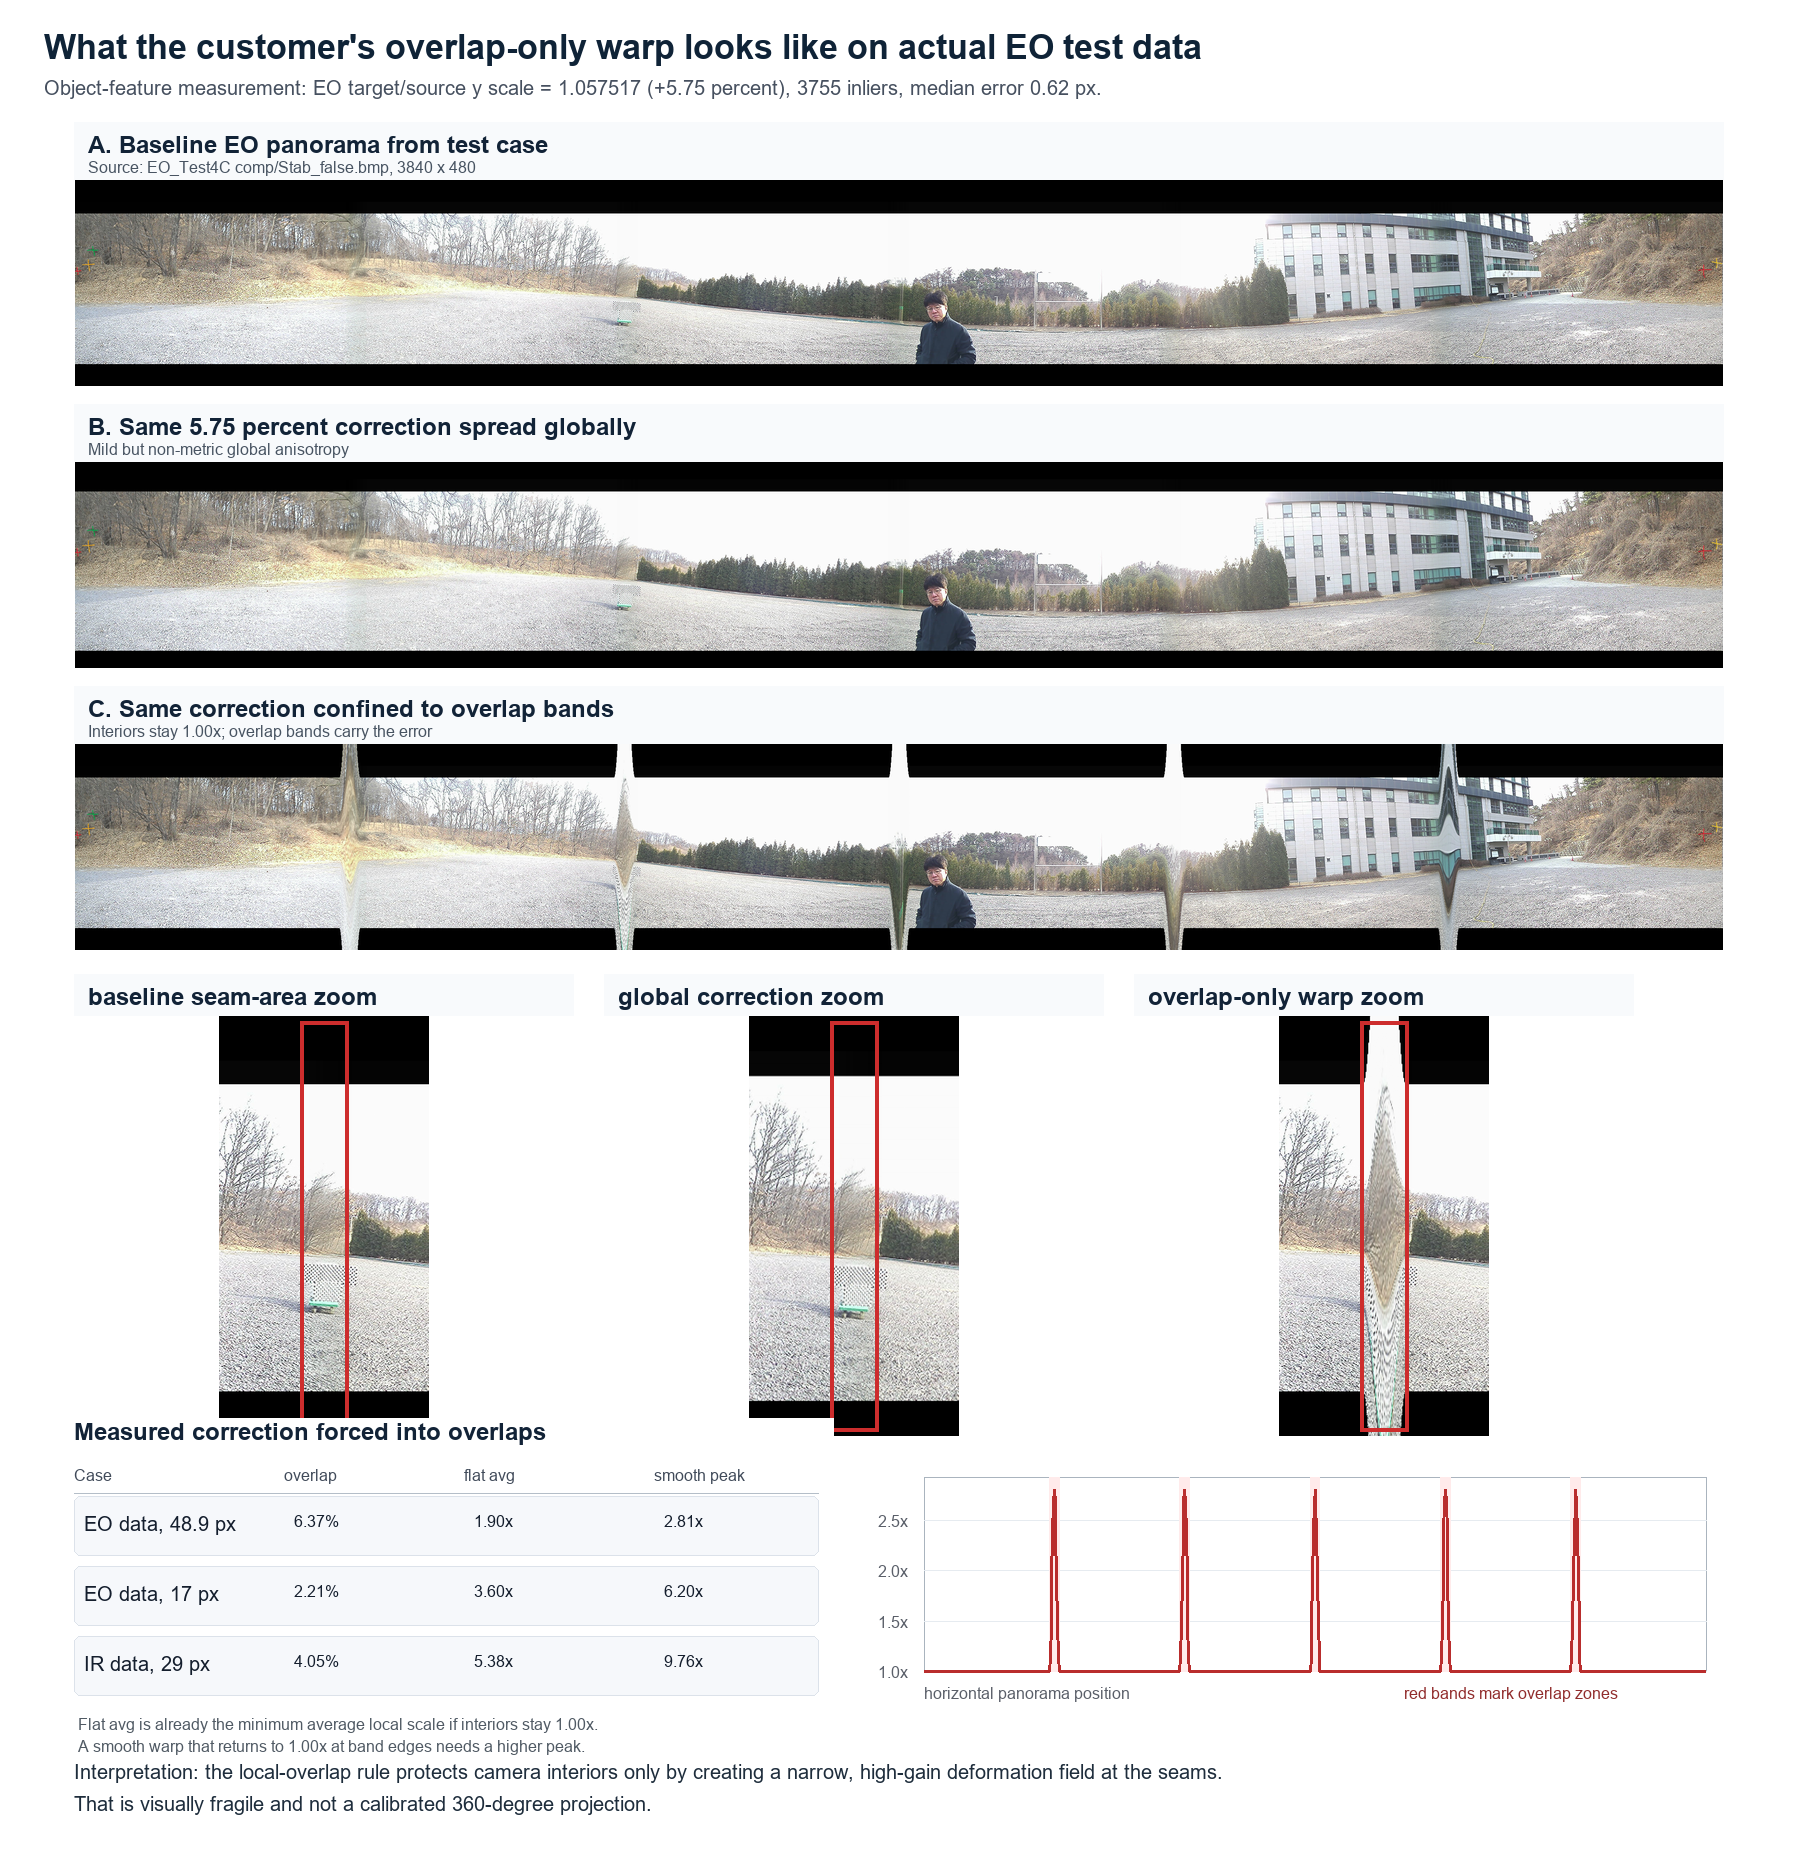
\includegraphics[width=\textwidth]{assets/customer_local_overlap_warp_demo.png}
\caption{Concrete simulation of the customer-proposed overlap-only correction on actual EO test-case imagery. The same measured EO correction that is mild when spread globally becomes a high-gain deformation field when camera interiors are held fixed and the correction is confined to the overlap bands. The visual result is seam-localized stretching/pinching, not preserved calibrated panorama geometry.}
\label{fig:local-overlap-demo}
\end{figure}

\subsection{Wider test: 25\% on each side of every tile}

The narrow-overlap result is clearly too severe for a useful display. A more practical interpretation is therefore tested: the correction is allowed to vary over the outer quarter of each tile on both sides, while the central half of every tile remains at scale $1.0$. For a tile width $T$ and side fraction $q=0.25$, the left and right support together occupy

\begin{equation}
f_{25}=2q=0.5
\end{equation}

of the complete panorama. At an internal seam, the right-side ramp of one tile and the left-side ramp of its neighbor form one continuous seam-centered zone of width $2qT$. The experiment uses a raised-cosine profile with zero slope where the ramp meets the protected tile center. The required scale values follow directly from Equations~\eqref{eq:overlapavg} and \eqref{eq:overlappeak}, replacing the physical-overlap fraction with $f_{25}=0.5$.

\begin{table}[H]
\centering
\caption{Measured correction distributed over the outer 25\% of both sides of each tile. EO uses six 640 px output sectors in the 3840 px unwrapped panorama. IR uses six 596 px sectors in its 3576 px unwrapped active panorama, corresponding to 1788 px in each folded half.}
\label{tab:quarter-tile}
\small
\begin{tabular}{@{}lrrrrr@{}}
\toprule
Case & Tile width & Ramp per side & Seam zone & Active-band average & Smooth peak \\
\midrule
EO measured $S_y=1.057517$ & 640 px & 160 px & 320 px & 1.115$\times$ & 1.230$\times$ \\
IR measured $S_y=1.177568$ & 596 px & 149 px & 298 px & 1.355$\times$ & 1.710$\times$ \\
\bottomrule
\end{tabular}
\end{table}

Figure~\ref{fig:quarter-tile-demo} shows that this wider field is materially better than the overlap-only case. In EO, the narrow high-gain pinch disappears and the transition becomes gradual enough to be considered for an operator-view prototype. This is a useful engineering result: the customer's underlying preference can be made visually plausible if ``local'' is expanded from the physical overlap to half of every output tile.

The wider support does not, however, make all four stated objectives simultaneous. EO vertical scale still changes continuously from $1.00\times$ at each tile center to $1.23\times$ at each seam; the corresponding IR range reaches $1.71\times$. Objects therefore change height and aspect ratio as they move through a ramp. The broad scallop visible at the upper and lower validity boundaries is equally important. Cropping that scallop to fill a rectangle discards a position-dependent amount of vertical field of view. Retaining all source rows leaves a non-rectangular or invalid boundary. Compressing the full source footprint into the rectangle keeps the rows but applies the same non-metric distortion in the opposite direction. The method can choose among these outcomes, but it cannot remove the tradeoff.

\begin{figure}[H]
\centering
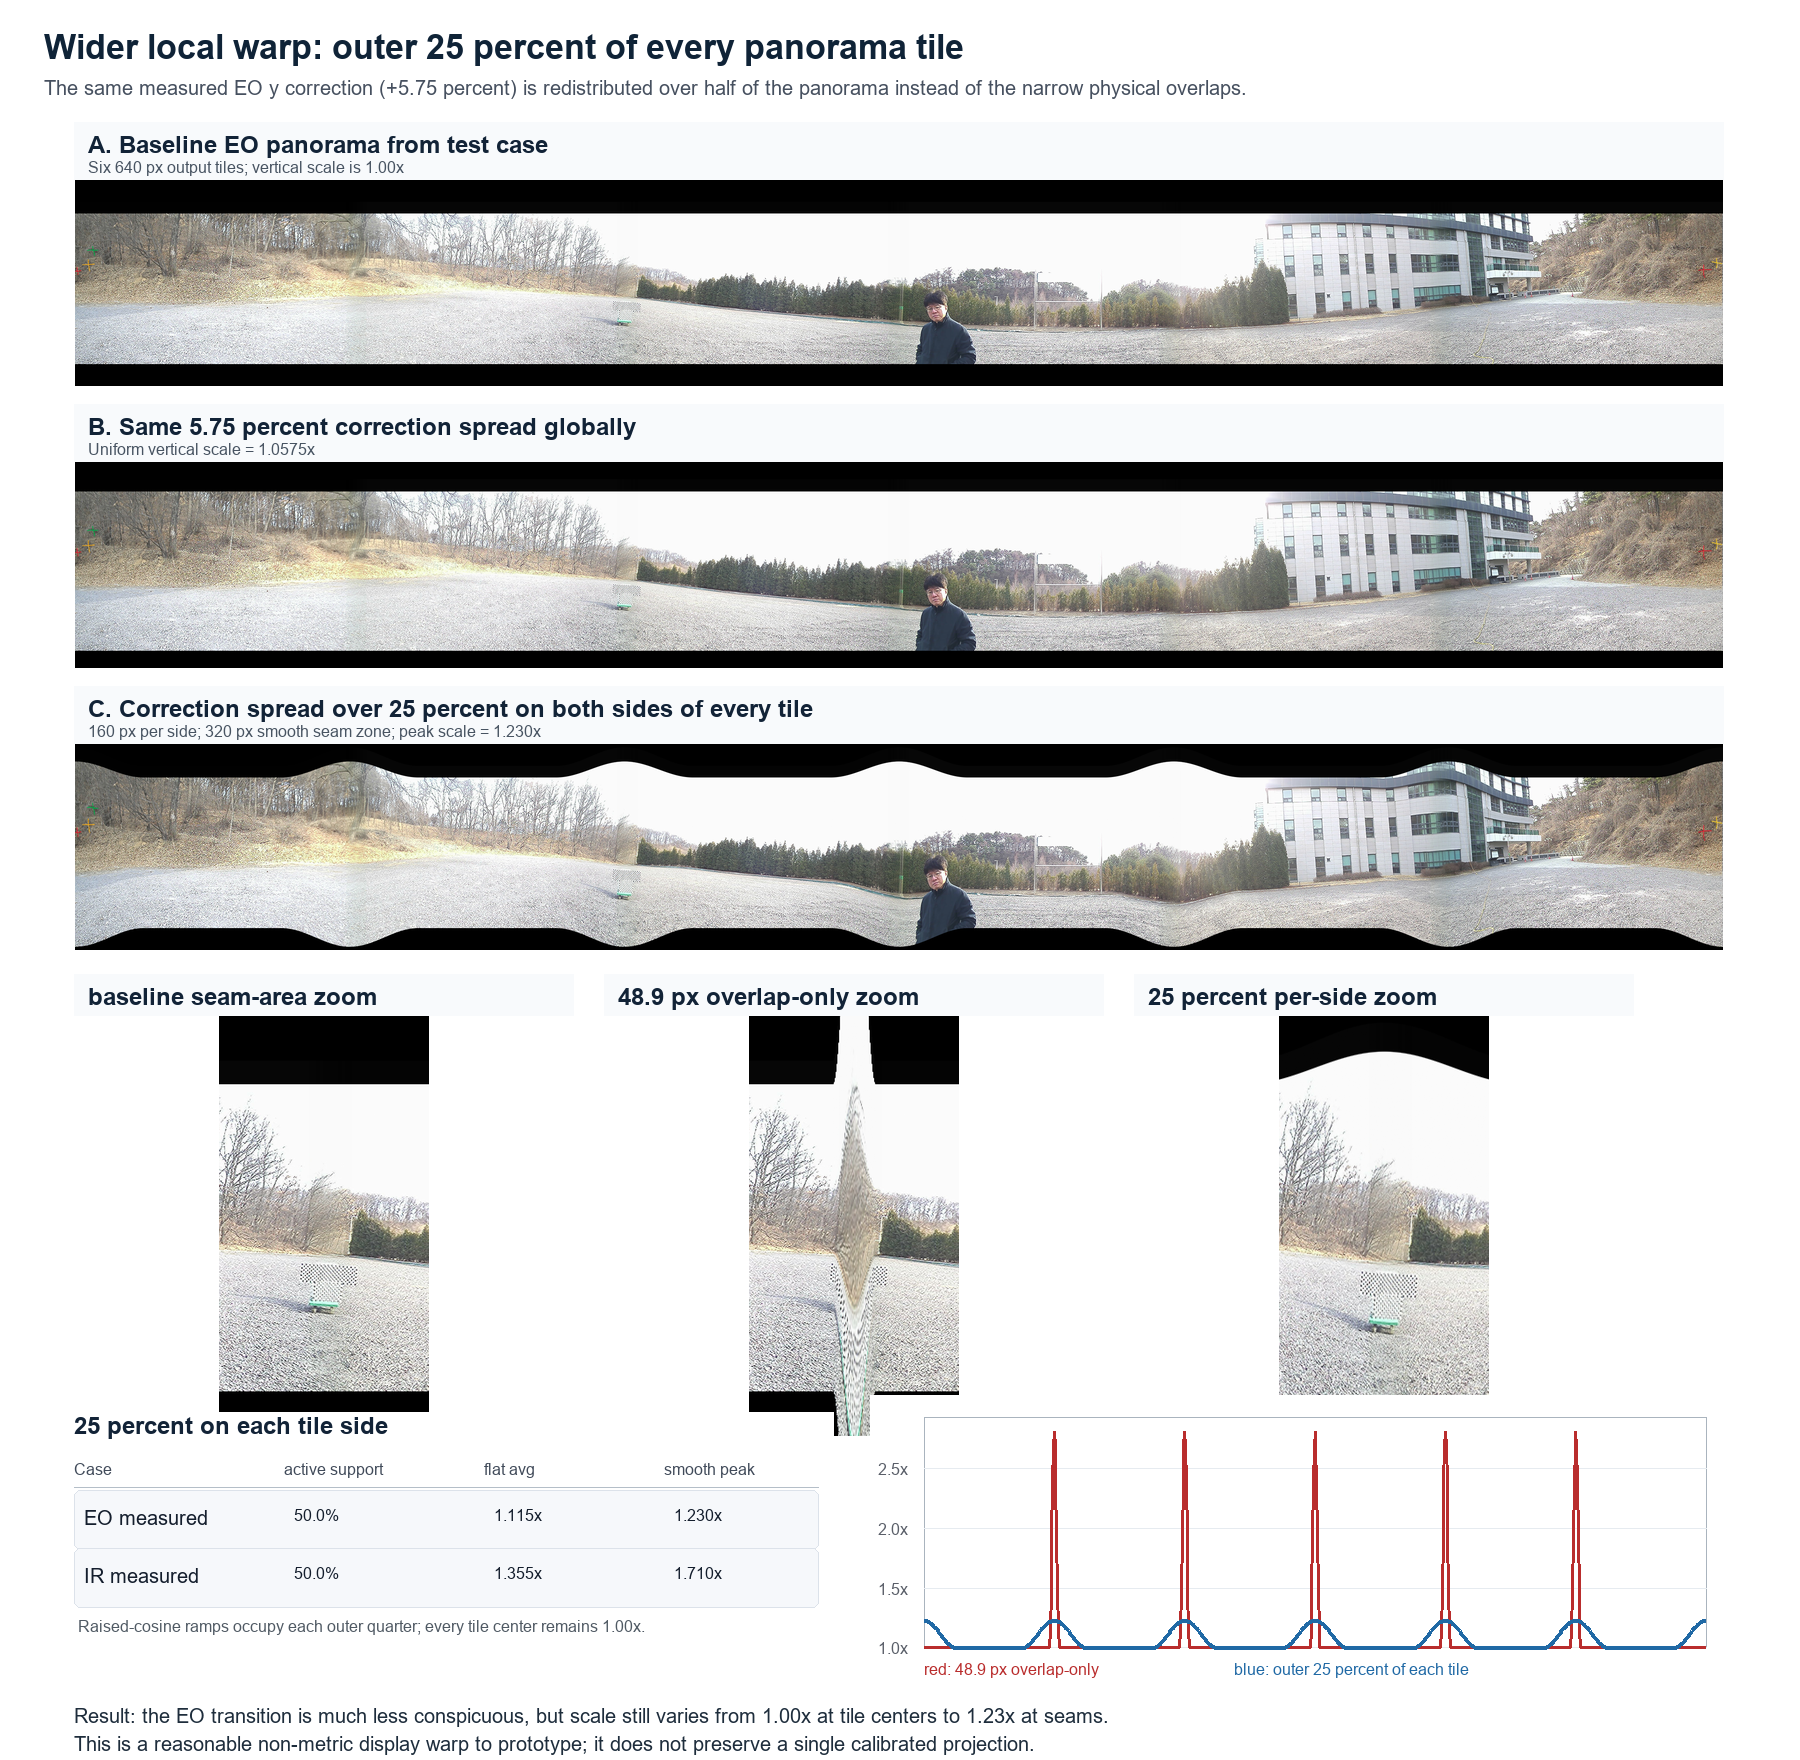
\includegraphics[width=\textwidth]{assets/customer_quarter_tile_warp_demo.png}
\caption{The measured EO correction redistributed over the outer 25\% of each side of every 640 px tile. Compared with the 48.9 px overlap-only simulation, the smooth 320 px seam zone reduces the peak scale from $2.81\times$ to $1.23\times$ and removes the visually extreme pinch. The remaining scalloped boundary and position-dependent object scale show why the result is a plausible non-metric display warp rather than a geometrically true rectangular panorama.}
\label{fig:quarter-tile-demo}
\end{figure}

\subsection{Further wider test: 37.5\% on each side}

The same experiment was repeated with the correction ramp covering the outer $q=0.375$ of both sides of every tile. The active support is therefore

\begin{equation}
f_{37.5}=2q=0.75,
\end{equation}

leaving only the central 25\% of each tile at scale $1.0$. For EO, each side ramp is 240 px and the combined seam-centered zone is 480 px wide. For IR, the corresponding ideal widths are 223.5 px per side and 447 px per seam zone.

\begin{table}[H]
\centering
\caption{Comparison of the two widened raised-cosine correction fields. Both preserve the measured panorama-average scale; widening support lowers peak deformation while reducing the undistorted camera interior.}
\label{tab:wide-tile-comparison}
\small
\begin{tabular}{@{}llrrrr@{}}
\toprule
Case & Side fraction & Active support & Undistorted center & Active-band average & Smooth peak \\
\midrule
EO, 25\% sides & 25\% & 50\% & 50\% & 1.115$\times$ & 1.230$\times$ \\
EO, 37.5\% sides & 37.5\% & 75\% & 25\% & 1.077$\times$ & 1.153$\times$ \\
IR, 25\% sides & 25\% & 50\% & 50\% & 1.355$\times$ & 1.710$\times$ \\
IR, 37.5\% sides & 37.5\% & 75\% & 25\% & 1.237$\times$ & 1.474$\times$ \\
\bottomrule
\end{tabular}
\end{table}

The 37.5\% result is visually gentler. In EO, the peak scale drops from $1.230\times$ to $1.153\times$, a one-third reduction in peak scale excess above unity. The upper and lower scallops become shallower, and the seam-area zoom approaches the baseline more closely. IR also improves, although a $1.474\times$ seam peak remains substantial.

This improvement does not come from recovering geometry; it comes from distributing the same correction over more pixels. Three quarters of every tile now have position-dependent vertical scale, and only a 160 px central strip of each 640 px EO sector remains undistorted. Thus 37.5\% is likely the more natural-looking operator view, while 25\% better preserves a larger camera interior. The choice is a perceptual tuning parameter between deformation amplitude and deformation extent, not a solution to the field-of-view constraint.

\begin{figure}[H]
\centering
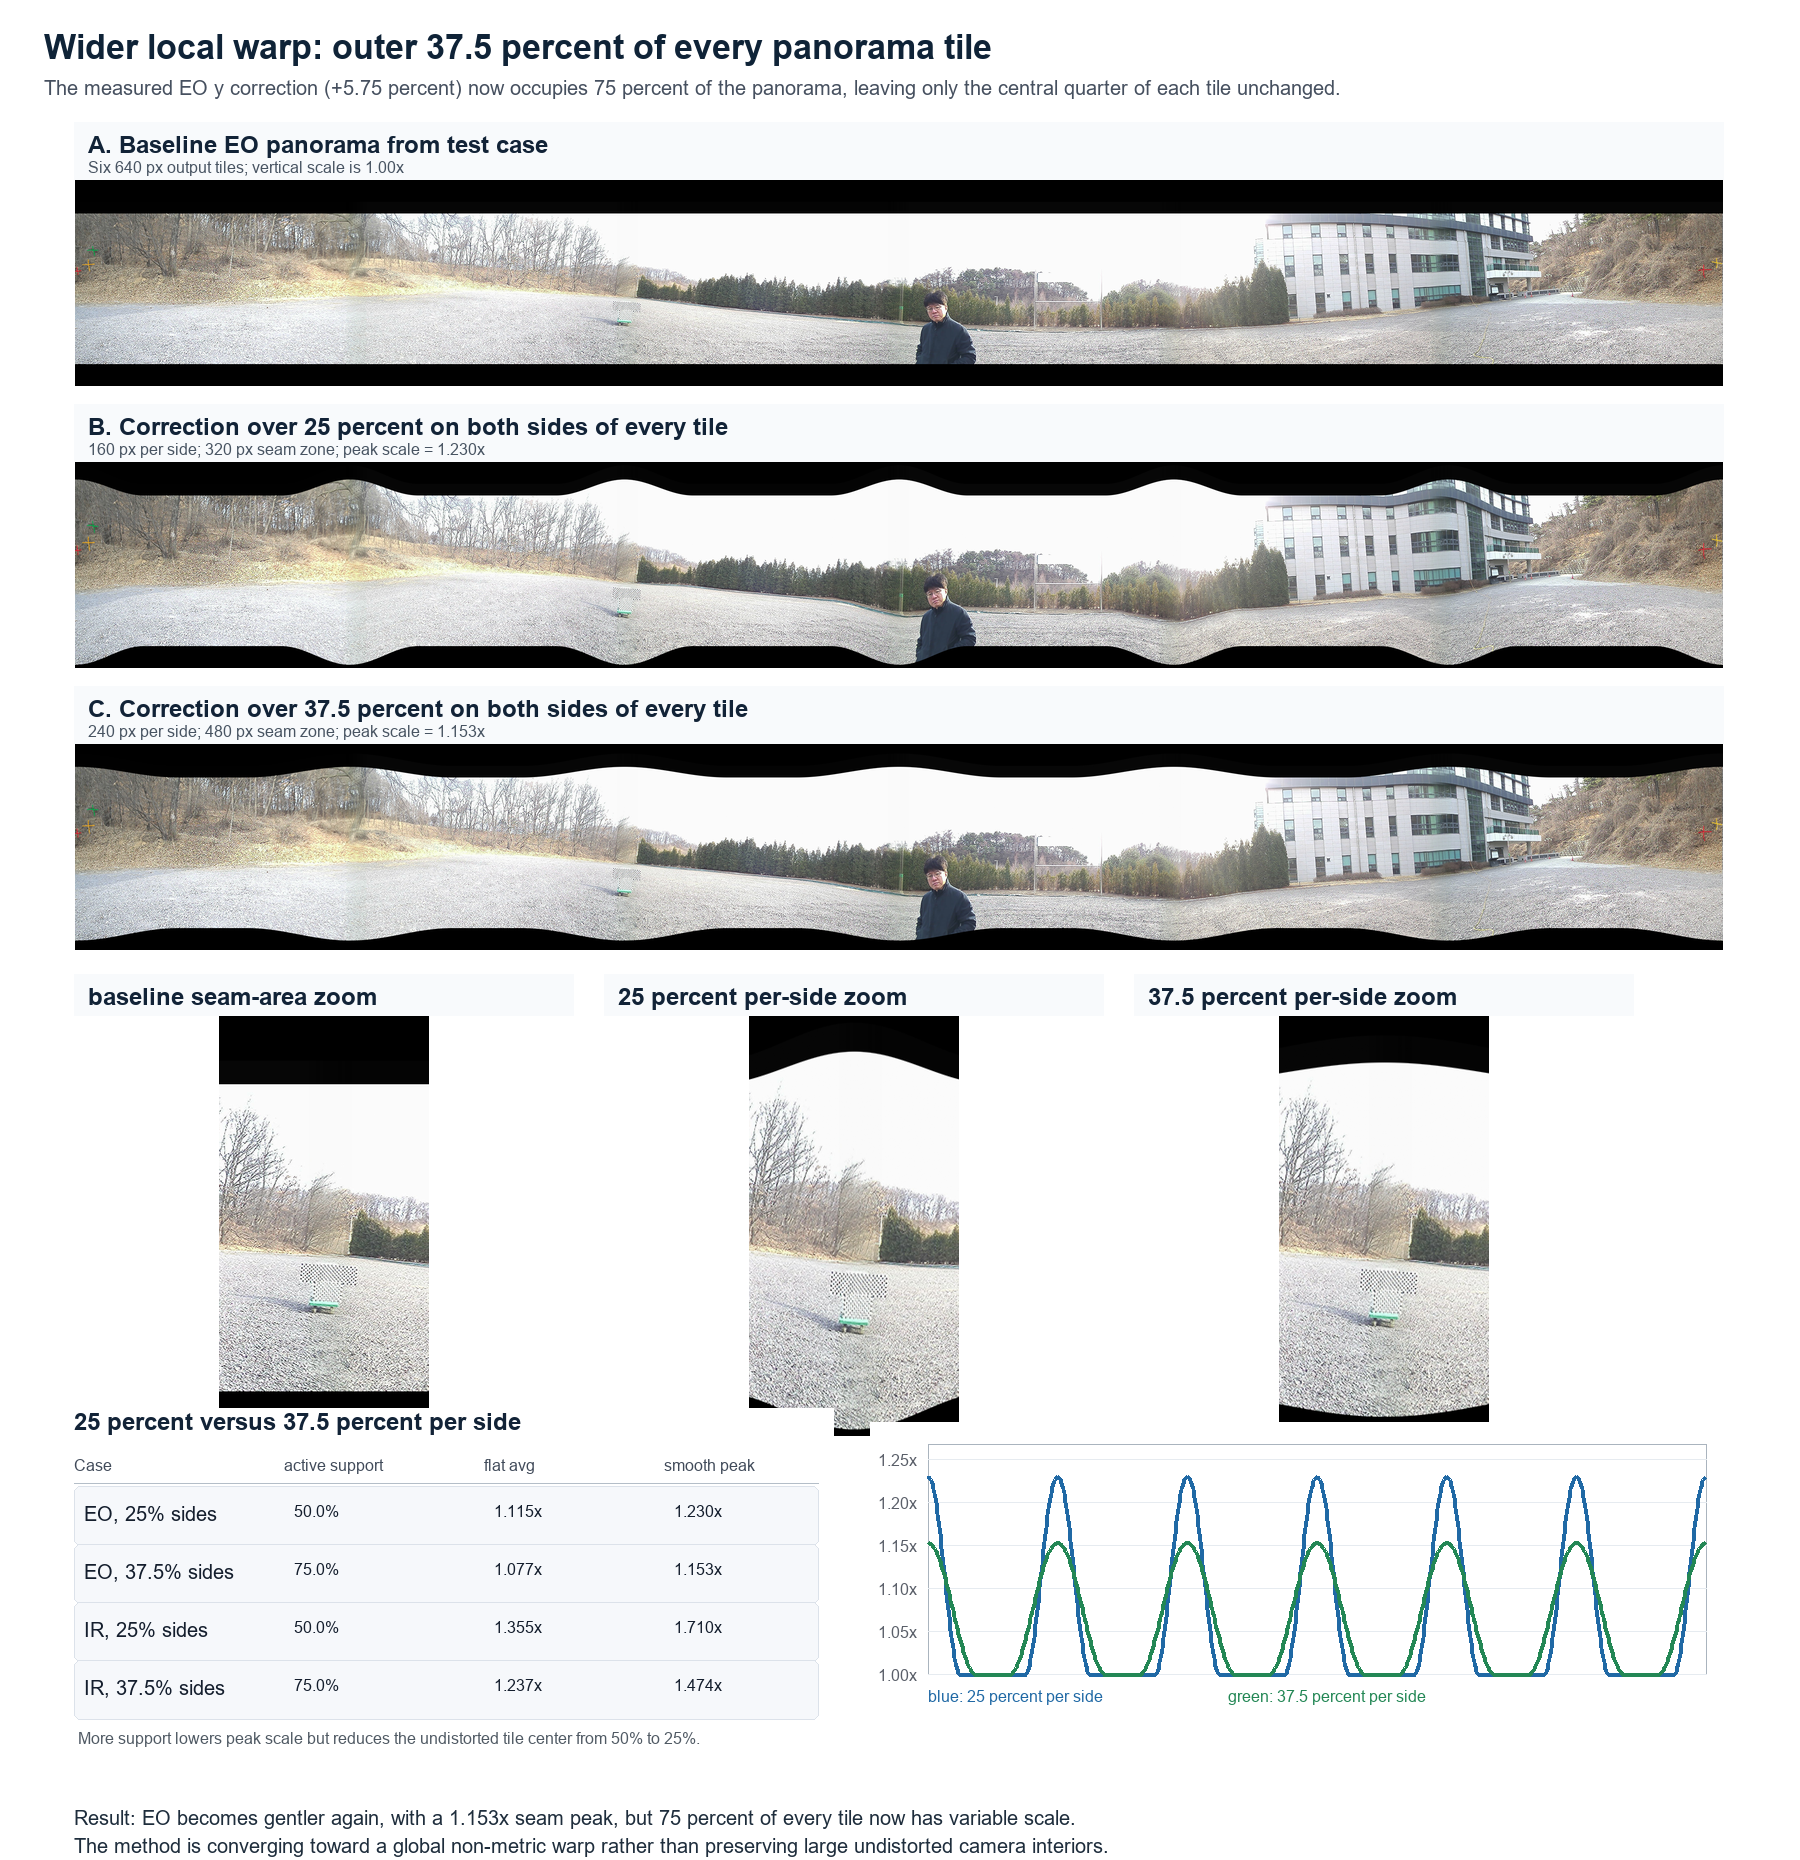
\includegraphics[width=\textwidth]{assets/customer_three_eighths_tile_warp_demo.png}
\caption{Measured EO correction distributed over the outer 37.5\% of each tile side and compared directly with the 25\% case. The 480 px EO seam zone lowers the smooth peak to $1.153\times$ and visibly reduces boundary scalloping. The correction now occupies 75\% of the panorama, demonstrating that the smoother appearance is obtained by spreading non-metric scale variation across most of each tile.}
\label{fig:three-eighths-tile-demo}
\end{figure}

\subsection{Implication for the projection choice}

The customer is correct that a non-cylindrical method can preserve more vertical source content for an operator display. The rigorous version of that idea is a calibrated multi-face or perspective-atlas representation, where each camera face keeps its own inverse ray model and the UI renders those faces on a 3-D surface. That approach does not pretend to be one rectangular cylindrical raster.

The proposed adaptive overlap warp is different. It uses a local two-dimensional deformation to make a rectangle look plausible. If the deformation is estimated from image features at runtime, it inherits the problems of feature-dependent still-image stitching: depth dependence, moving-object sensitivity, and seam shimmer. If a wider 25\% or 37.5\% tile-edge deformation is instead calibrated offline and held fixed, those temporal estimation problems are avoided and the map is compatible with deterministic FPGA lookup. The remaining limitation is geometric: scale depends on azimuth and there is no single projection model or stable global pixel-to-ray interpretation. The fixed wider warp can be offered as an optional operator view, but it should not replace the metric cylindrical mode used for measurement, stabilization, tracking, and downstream analytics.

\section{Practical Alternatives for the Existing Hardware}

\subsection{Metric flat panorama}

For a single flat panorama in which every output pixel has a well-defined global ray, retain the calibrated cylindrical or equirectangular map. The output must then use one of two honest representations:

\begin{itemize}
  \item crop to the vertical range valid at every azimuth; or
  \item retain the curved/scalloped validity boundary and encode unavailable regions as black or masked pixels.
\end{itemize}

This is the appropriate mode for measurement, tracking, target localization, and any downstream algorithm that depends on angular consistency.

\subsection{Perspective atlas rendered by the UI}

With the existing six cameras, the full sensor footprint can be retained as six calibrated rectilinear faces, analogous to a cubemap or a hexagonal-prism atlas. Each face preserves its source rays and may be packed into an HD transport frame. The UI then renders the faces on their corresponding 3-D surfaces.

This representation is geometrically valid as a multi-face atlas and preserves substantially more vertical sensor content. It is not one uniform cylindrical raster: horizontal angular sampling varies within each perspective face, and the UI or analytics layer must use the face-specific inverse projection. The current precomputed-map and RowRun architecture could support such a mode through different offline maps, provided row-span and memory bounds are reverified.

\subsection{Optical overscan}

If the requirement is simultaneously a full-height rectangle, one global angular projection, and no invalid top/bottom regions, additional optical coverage is required. For the EO numbers above, a vertical field near $58^\circ$ is the theoretical minimum for a $\pm30^\circ$ sector before allowing calibration tolerance, stabilization margin, lens distortion, and assembly error. A practical design would require additional margin beyond that minimum.

\subsection{Optional non-metric operator view}

A ratio-preserving, mesh-rectangled, or column-normalized warp can be offered as an optional human-view mode. Because the existing FPGA uses offline base maps and a generic fixed-point renderer, a selected non-metric warp could be precomputed and translated into the same map/RowRun representation. It should be explicitly labeled as a display projection and should not replace the calibrated mode used for measurement or machine analysis.

\section{Assessment of the Existing G-Locked System}

\subsection{Architectural correspondence to the actual requirement}

The internal C reference implementation and manuscript describe a fundamentally different control structure from the reviewed work \cite{glocked,internalc}:

\begin{itemize}
  \item lens undistortion and cylindrical projection are composed offline into stable source-coordinate base maps;
  \item per-frame motion is supplied by the IMU rather than rediscovered from scene features;
  \item runtime correction is reduced to per-camera Q1.15 sine/cosine terms and a fixed-point vertical shift;
  \item destination samples are grouped by source-row bucket and compressed into piecewise-linear RowRuns;
  \item each camera renderer requires only two source lines at a time; and
  \item random destination writes are bounded inside an on-chip RowWindow, while DDR access remains burst-oriented.
\end{itemize}

This architecture corresponds directly to the fixed-rig, video-rate problem. The scene-independent calibration also generalizes naturally to IR, where visible-light feature networks or SIFT-based runtime matching may fail.

\subsection{Current routed implementation evidence}

The current XCKU15P routed checkpoint provides hardware evidence absent from both reviewed papers. The timing report closes the main $233.38$ MHz clock with setup, hold, and pulse-width margins all positive. There are zero failing setup or hold endpoints and zero routing errors \cite{vivado}.

\begin{table}[ht]
\centering
\caption{Current full-design post-route snapshot. Utilization includes the complete system, including camera interfaces, DDR/MIG, HD-SDI path, control, buffers, and restored debug infrastructure; it is not a renderer-only figure.}
\label{tab:fpga}
\small
\begin{tabular}{@{}lrrr@{}}
\toprule
Resource or timing item & Used / value & Available & Utilization \\
\midrule
CLB LUTs & 48,095 & 522,720 & 9.20\% \\
CLB registers & 77,034 & 1,045,440 & 7.37\% \\
Block RAM tiles & 778.5 & 984 & 79.12\% \\
UltraRAM & 10 & 128 & 7.81\% \\
DSP48E2 & 26 & 1,968 & 1.32\% \\
\midrule
Worst setup slack & $0.055$ ns & --- & Pass \\
Worst hold slack & $0.010$ ns & --- & Pass \\
Worst pulse-width slack & $0.047$ ns & --- & Pass \\
Routable nets with errors & 0 & 137,206 routed & Pass \\
\bottomrule
\end{tabular}
\end{table}

The manuscript's approximately 1.93 MB value is an analytical working-set estimate for the panorama renderer's two-line caches, active RowWindow, and slice ping-pong buffers. It should not be presented as the total placed-device memory utilization. The full bitstream uses 79.12\% of BRAM tiles because the complete system contains additional video, DDR, interface, buffering, and debug structures. Reporting both figures will make the hardware claim substantially more credible.

\section{Conclusion}

The reviewed literature does not justify replacing the existing calibrated cylindrical projection. Xu \emph{et al.} propose a useful perceptual still-image warp, but their output is a piecewise, scene-dependent composition rather than a single metric projection; the total measured rate is below one image pair per second, and there is no multi-camera, video, infrared, closure, or hardware validation. Wang \emph{et al.} solve stereoscopic disparity and naturalness using an even more elaborate iterative feature/mesh pipeline, with no cylindrical projection or runtime evidence.

The vertical-field limitation is dictated by pinhole-ray geometry. At the edge of a $60^\circ$ camera sector, a $51.3^\circ$-vertical EO sensor provides approximately $45.2^\circ$ of common elevation. Filling a full-height rectangle without crop or invalid pixels therefore requires either additional optical vertical coverage or a non-metric deformation. A visually pleasing rectangle is achievable; a geometrically true rectangle containing uncaptured rays is not.

For the existing hardware, the defensible engineering choices are: retain the calibrated cylindrical map for metric operation; optionally expose a masked full-footprint or multi-face perspective atlas; add optical overscan when a full-height metric rectangle is mandatory; and reserve adaptive ratio-preserving or fixed wide tile-edge warps for clearly labeled operator-view modes. The new tests indicate that fixed 25\% and 37.5\% variants are credible display prototypes because they lower the measured EO peak scale to $1.230\times$ and $1.153\times$, respectively, without requiring runtime feature estimation. The 37.5\% case is smoother but applies variable scale to 75\% of every tile.

\begin{center}
\fcolorbox{navy}{lightblue}{%
\begin{minipage}{0.91\textwidth}
\textbf{Customer-facing technical conclusion.}

The cited work performs perceptual rectangling of still-image pairs using scene-dependent two-dimensional warps. It neither preserves calibrated ray geometry nor recovers the vertical rays absent at sensor corners, and it provides no six-camera, 360-degree, video, thermal, or FPGA validation. Measured EO/IR data show that correction confined to physical overlaps produces unusably high local scale. Expanding the correction to the outer 25\% and 37.5\% of each tile side improves the EO result substantially, reducing the smooth peak to $1.230\times$ and $1.153\times$, and is credible as a fixed non-metric operator-view mode. The smoother 37.5\% case changes scale over 75\% of each tile. Both variants still vary object scale with azimuth and must either crop the scalloped boundary, retain invalid pixels, or compress the source footprint. A geometrically true full-height rectangle requires additional vertical optical coverage or a masked/multi-face output representation.
\end{minipage}}
\end{center}

\begin{thebibliography}{99}
\small

\bibitem{xu2018}
Y. Xu, J. Chen, and T. Liao, ``Ratio-Preserving Half-Cylindrical Warps for Natural Image Stitching,'' arXiv:1803.06655, 2018. Available: \url{https://arxiv.org/abs/1803.06655}

\bibitem{wang2018}
H. Wang, Y. Zhou, X. Wang, and L. Fang, ``A Natural Shape-Preserving Stereoscopic Image Stitching,'' in \emph{Proc. IEEE ICASSP}, 2018, pp. 1812--1816, doi: 10.1109/ICASSP.2018.8461411.

\bibitem{kang2019}
L. Kang, Y. Wei, J. Jiang, and Y. Xie, ``Robust Cylindrical Panorama Stitching for Low-Texture Scenes Based on Image Alignment Using Deep Learning and Iterative Optimization,'' \emph{Sensors}, vol. 19, no. 23, art. 5310, 2019, doi: 10.3390/s19235310.

\bibitem{zhang2019}
Y. Zhang, Y.-K. Lai, and F.-L. Zhang, ``Stereoscopic Image Stitching with Rectangular Boundaries,'' \emph{The Visual Computer}, vol. 35, pp. 823--835, 2019, doi: 10.1007/s00371-019-01694-7.

\bibitem{yan2020}
W. Yan, G. Yue, J. Xu, Y. Yu, K. Wang, C. Tang, and X. Tong, ``Shape-Optimizing Mesh Warping Method for Stereoscopic Panorama Stitching,'' \emph{Information Sciences}, vol. 511, pp. 58--73, 2020, doi: 10.1016/j.ins.2019.09.051.

\bibitem{chen2020}
K. Chen, J. Yao, J. Tu, Y. Liu, Y. Li, and L. Li, ``Vanishing Point Guided Natural Image Stitching,'' arXiv:2004.02478, 2020. Available: \url{https://arxiv.org/abs/2004.02478}

\bibitem{nam2021}
D.-Y. Nam and J.-K. Han, ``An Efficient Algorithm for Generating Harmonized Stereoscopic 360-Degree VR Images,'' \emph{IEEE Trans. Circuits Syst. Video Technol.}, 2021, doi: 10.1109/TCSVT.2021.3056065.

\bibitem{brown2007}
M. Brown and D. G. Lowe, ``Automatic Panoramic Image Stitching Using Invariant Features,'' \emph{Int. J. Comput. Vis.}, vol. 74, no. 1, pp. 59--73, 2007.

\bibitem{chang2014}
C.-H. Chang, Y. Sato, and Y.-Y. Chuang, ``Shape-Preserving Half-Projective Warps for Image Stitching,'' in \emph{Proc. IEEE CVPR}, 2014, pp. 3254--3261.

\bibitem{szeliski1997}
R. Szeliski and H.-Y. Shum, ``Creating Full View Panoramic Image Mosaics and Environment Maps,'' in \emph{Proc. ACM SIGGRAPH}, 1997, pp. 251--258.

\bibitem{glocked}
M. Awais and Y. Hwang, ``G-Locked Panorama Stabilization: A Streaming IMU-Locked Algorithm for Real-Time Cylindrical Panorama Stabilization and FPGA-Oriented Deployment,'' internal manuscript, 2026. Source: \path{C:/SVNProjects/IMU_Stabilize_v40/Paper_Latex/Panorama_Stabilization_Article (1)/g_locked_panorama_stabilization.tex}.

\bibitem{internalc}
M. Awais, ``IMU Stabilize GYRO V19 Reference Implementation,'' internal C/C++ implementation, 2026. Source: \path{C:/SVNProjects/IMU_Stabilize_v40/IMU_stabilize_GYRO/IMU_stabilize_GYRO.cpp}.

\bibitem{testcases}
M. Awais, ``EO/IR Panorama Stabilization Test Cases and Object-Based Stretch Analysis,'' internal dataset and derived measurements, 2026. Source: \path{C:/SVNProjects/IMU_Stabilize_v40/EO_IR_TestCases/}.

\bibitem{vivado}
AMD Vivado, ``KintexTop EO/IR HD-SDI Panorama Base: Routed Timing and Route-Status Reports,'' XCKU15P implementation build, 11 August 2026. Source: \path{E:/Xylinx/EO_Panorama_V19_M1/EO_Panorama_V19_M1.runs/impl_1/}.

\bibitem{openalex}
OpenAlex, bibliographic records W2793335423 and W2890038543, accessed 12 August 2026. Available: \url{https://openalex.org/}

\bibitem{pwc}
Papers With Code, author and implementation index for Yifang Xu, accessed 12 August 2026. Available: \url{https://paperswithcode.com/author/yifang-xu}

\end{thebibliography}

\end{document}
